\chapter{~\LaTeX~的安装}

~\LaTeX~的使用需要安装相关的软件,目前主要使用的有两种方式进行~\LaTeX~编辑:
\begin{itemize}
  \item 在线编辑器(Overleaf、TeXPage)
  \item 本地编辑器(VSCode+插件、TeXShop)
\end{itemize}

个人推荐使用Overleaf进行编辑,无需安装本地编译环境,同时还可以进行多人协同操作。但使用在线编辑器的缺点就是必须连接网络。

\section{Overleaf的使用}

进入到Overleaf首页:\url{https://www.overleaf.com},点击右上角Register注册新账户。登录成功后如图\ref{fig:2-overlead-home}所示,会进入到项目界面。

\begin{figure}[htb]
  \centering
  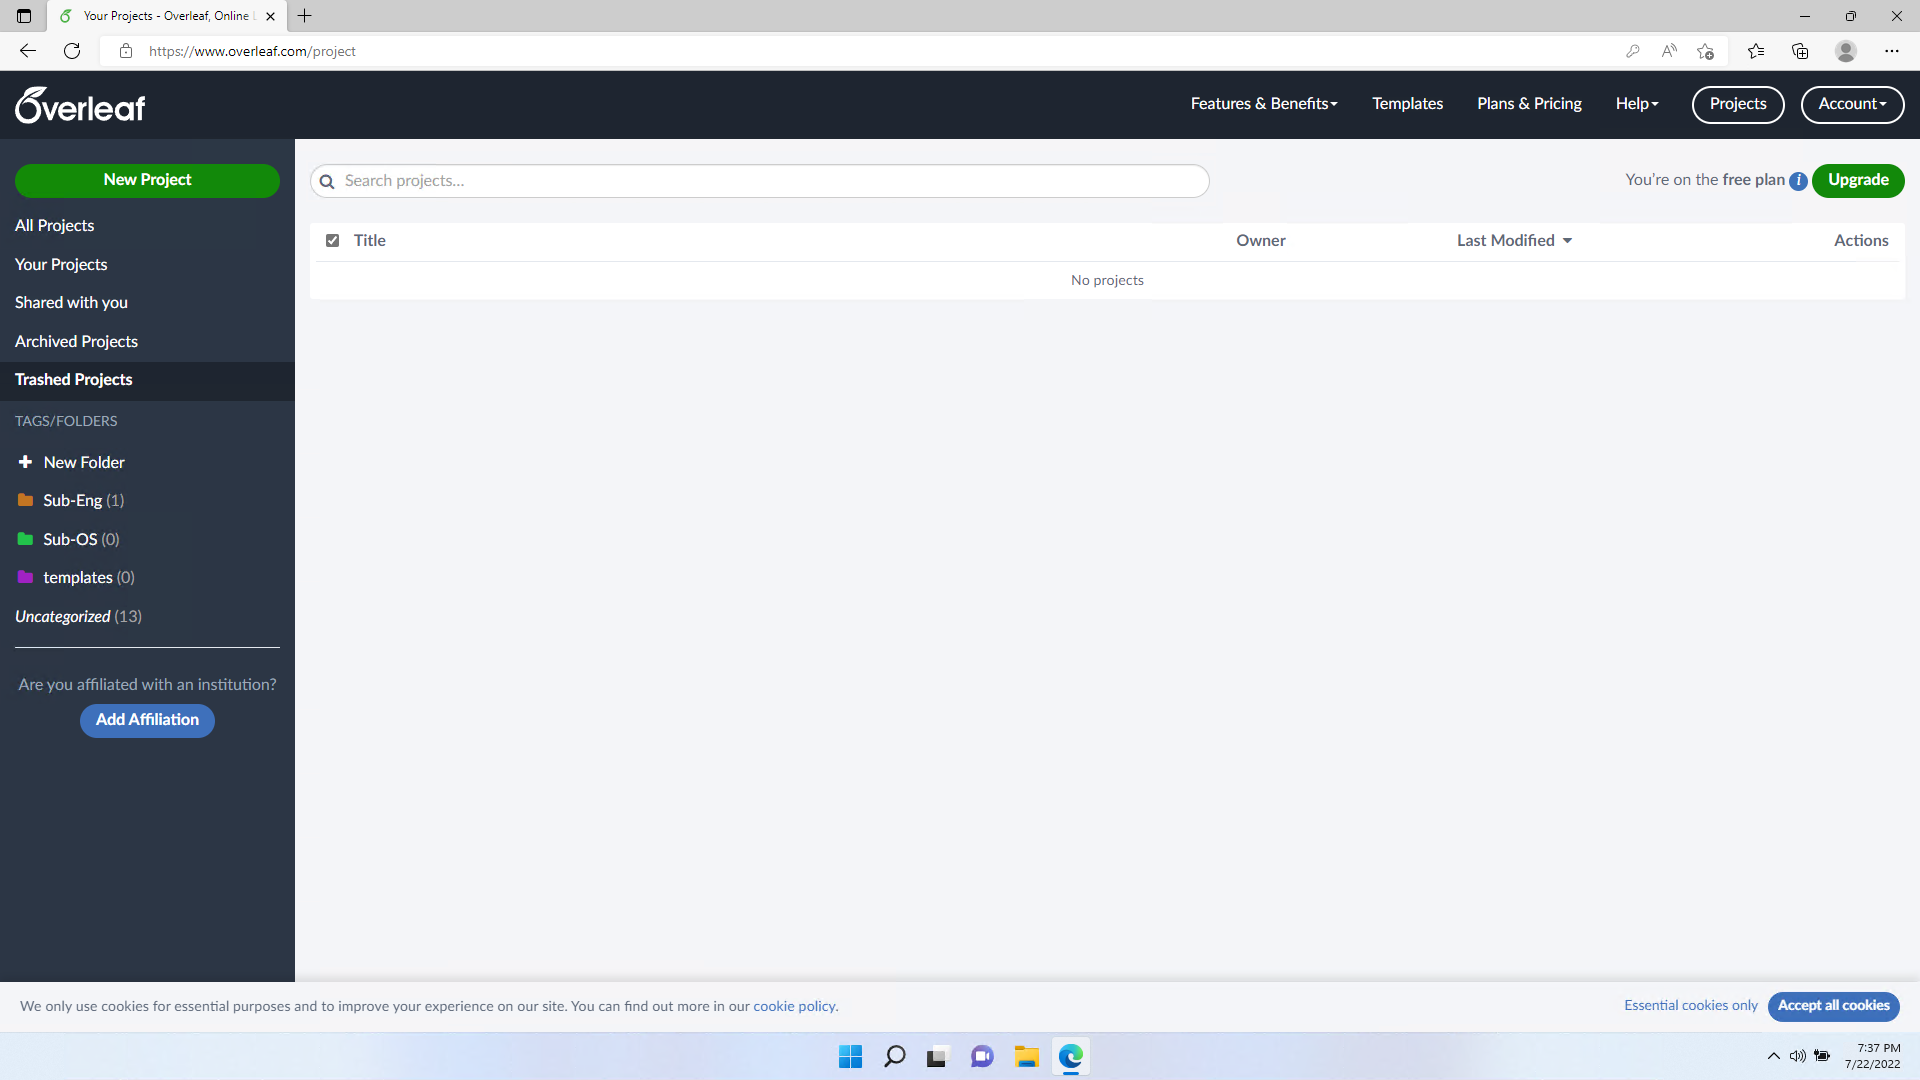
\includegraphics[width=0.9\textwidth]{figures/chapter2/overleaf-home.png}
  \caption{Overleaf项目页面}
  \label{fig:2-overlead-home}
\end{figure}

此时你需要将使用的模板下载至本地。以此项目为例,进入\url{https://github.com/Nagico/WHUExperiment},点击Download ZIP即可将模板下载到本地。该模板同时也一同放至本文档旁,可以直接使用,但仍建议从Github上下载最新版本的模板。

\begin{figure}[htb]
    \centering
    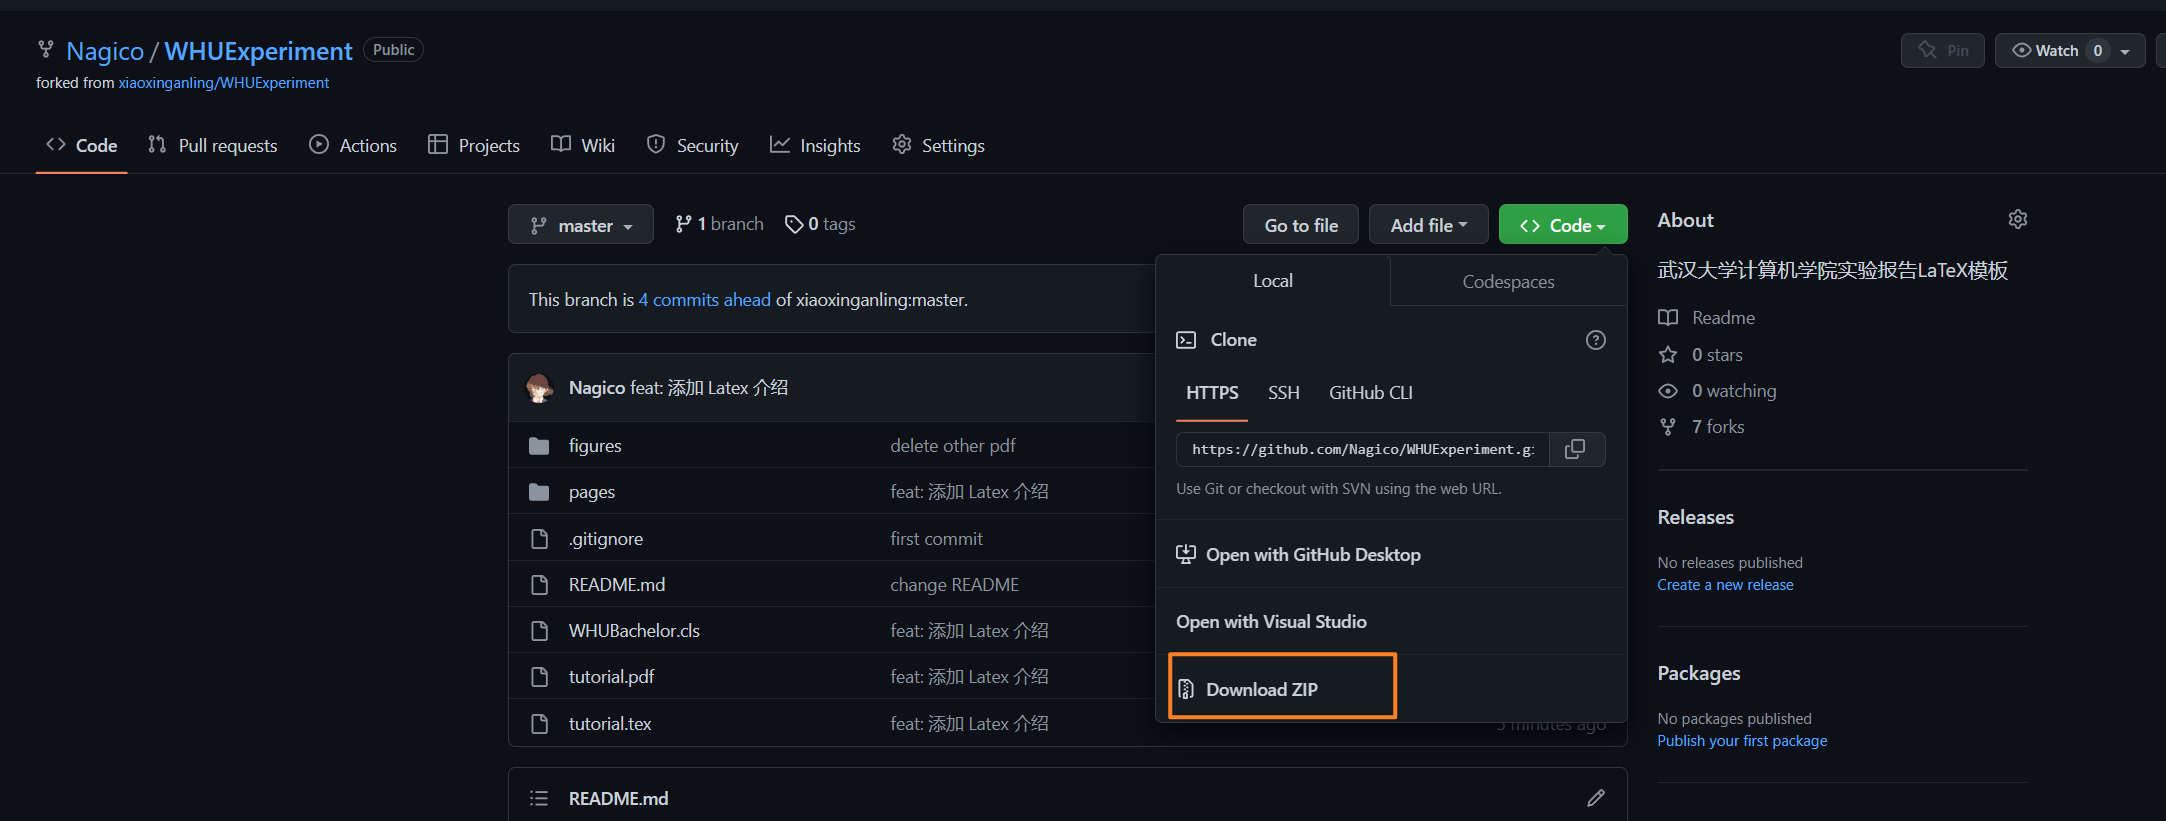
\includegraphics[width=0.95\textwidth]{figures/chapter2/download-repo.png}
    \caption{下载模板}
    \label{fig:2-github-download}
\end{figure}

在Overleaf页面点击左侧的New Project,选择Upload Project,将下载的ZIP文件上传,即可将模板导入至Overleaf。

\begin{figure}[htb]
  \centering
  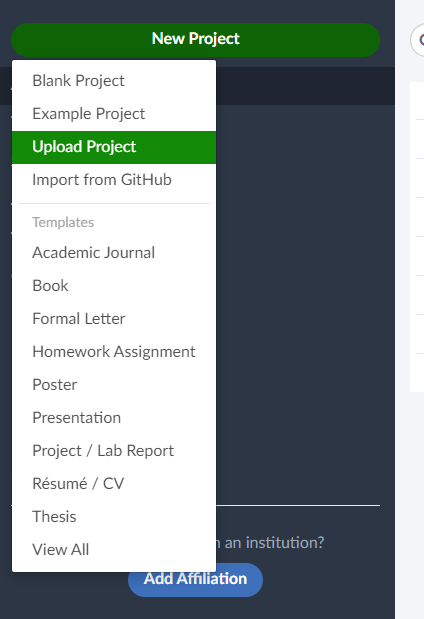
\includegraphics[width=0.3\textwidth]{figures/chapter2/upload-project.png}
  \caption{导入模板}
  \label{fig:2-upload-project}
\end{figure}

导入后会自动跳转到编辑界面,需要点击左上角的Menu进入设置界面,将Compiler修改为XeLatex以支持中文(图\ref{fig:2-compiler})。

\begin{figure}[H]
  \centering
  \begin{subfigure}{0.55\textwidth}
    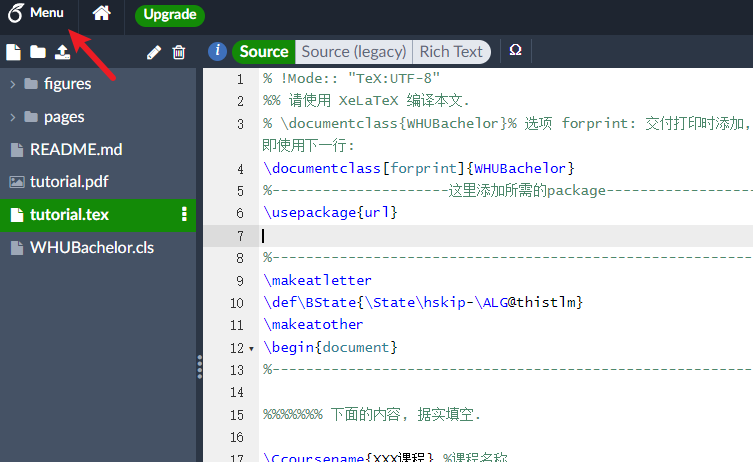
\includegraphics[width=\linewidth]{figures/chapter2/menu.png}
    \caption{Menu按钮}
    \label{fig:2-menu}
  \end{subfigure}\qquad
  \begin{subfigure}{0.3\textwidth}
    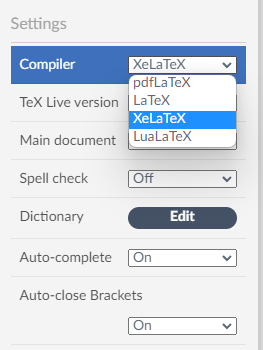
\includegraphics[width=\linewidth]{figures/chapter2/xelatex.png}
    \caption{选择Compiler}
    \label{fig:2-compiler}
  \end{subfigure}
  \caption{配置~\LaTeX~}
  \label{fig:2-latex-conf}
\end{figure}

修改成功后点击Recompile重新编辑,即可正常使用。你可以在左侧进行项目文件的管理,后续所需的图片可以在相应文件夹处右键,选择Upload上传。

\begin{figure}[htb]
  \centering
  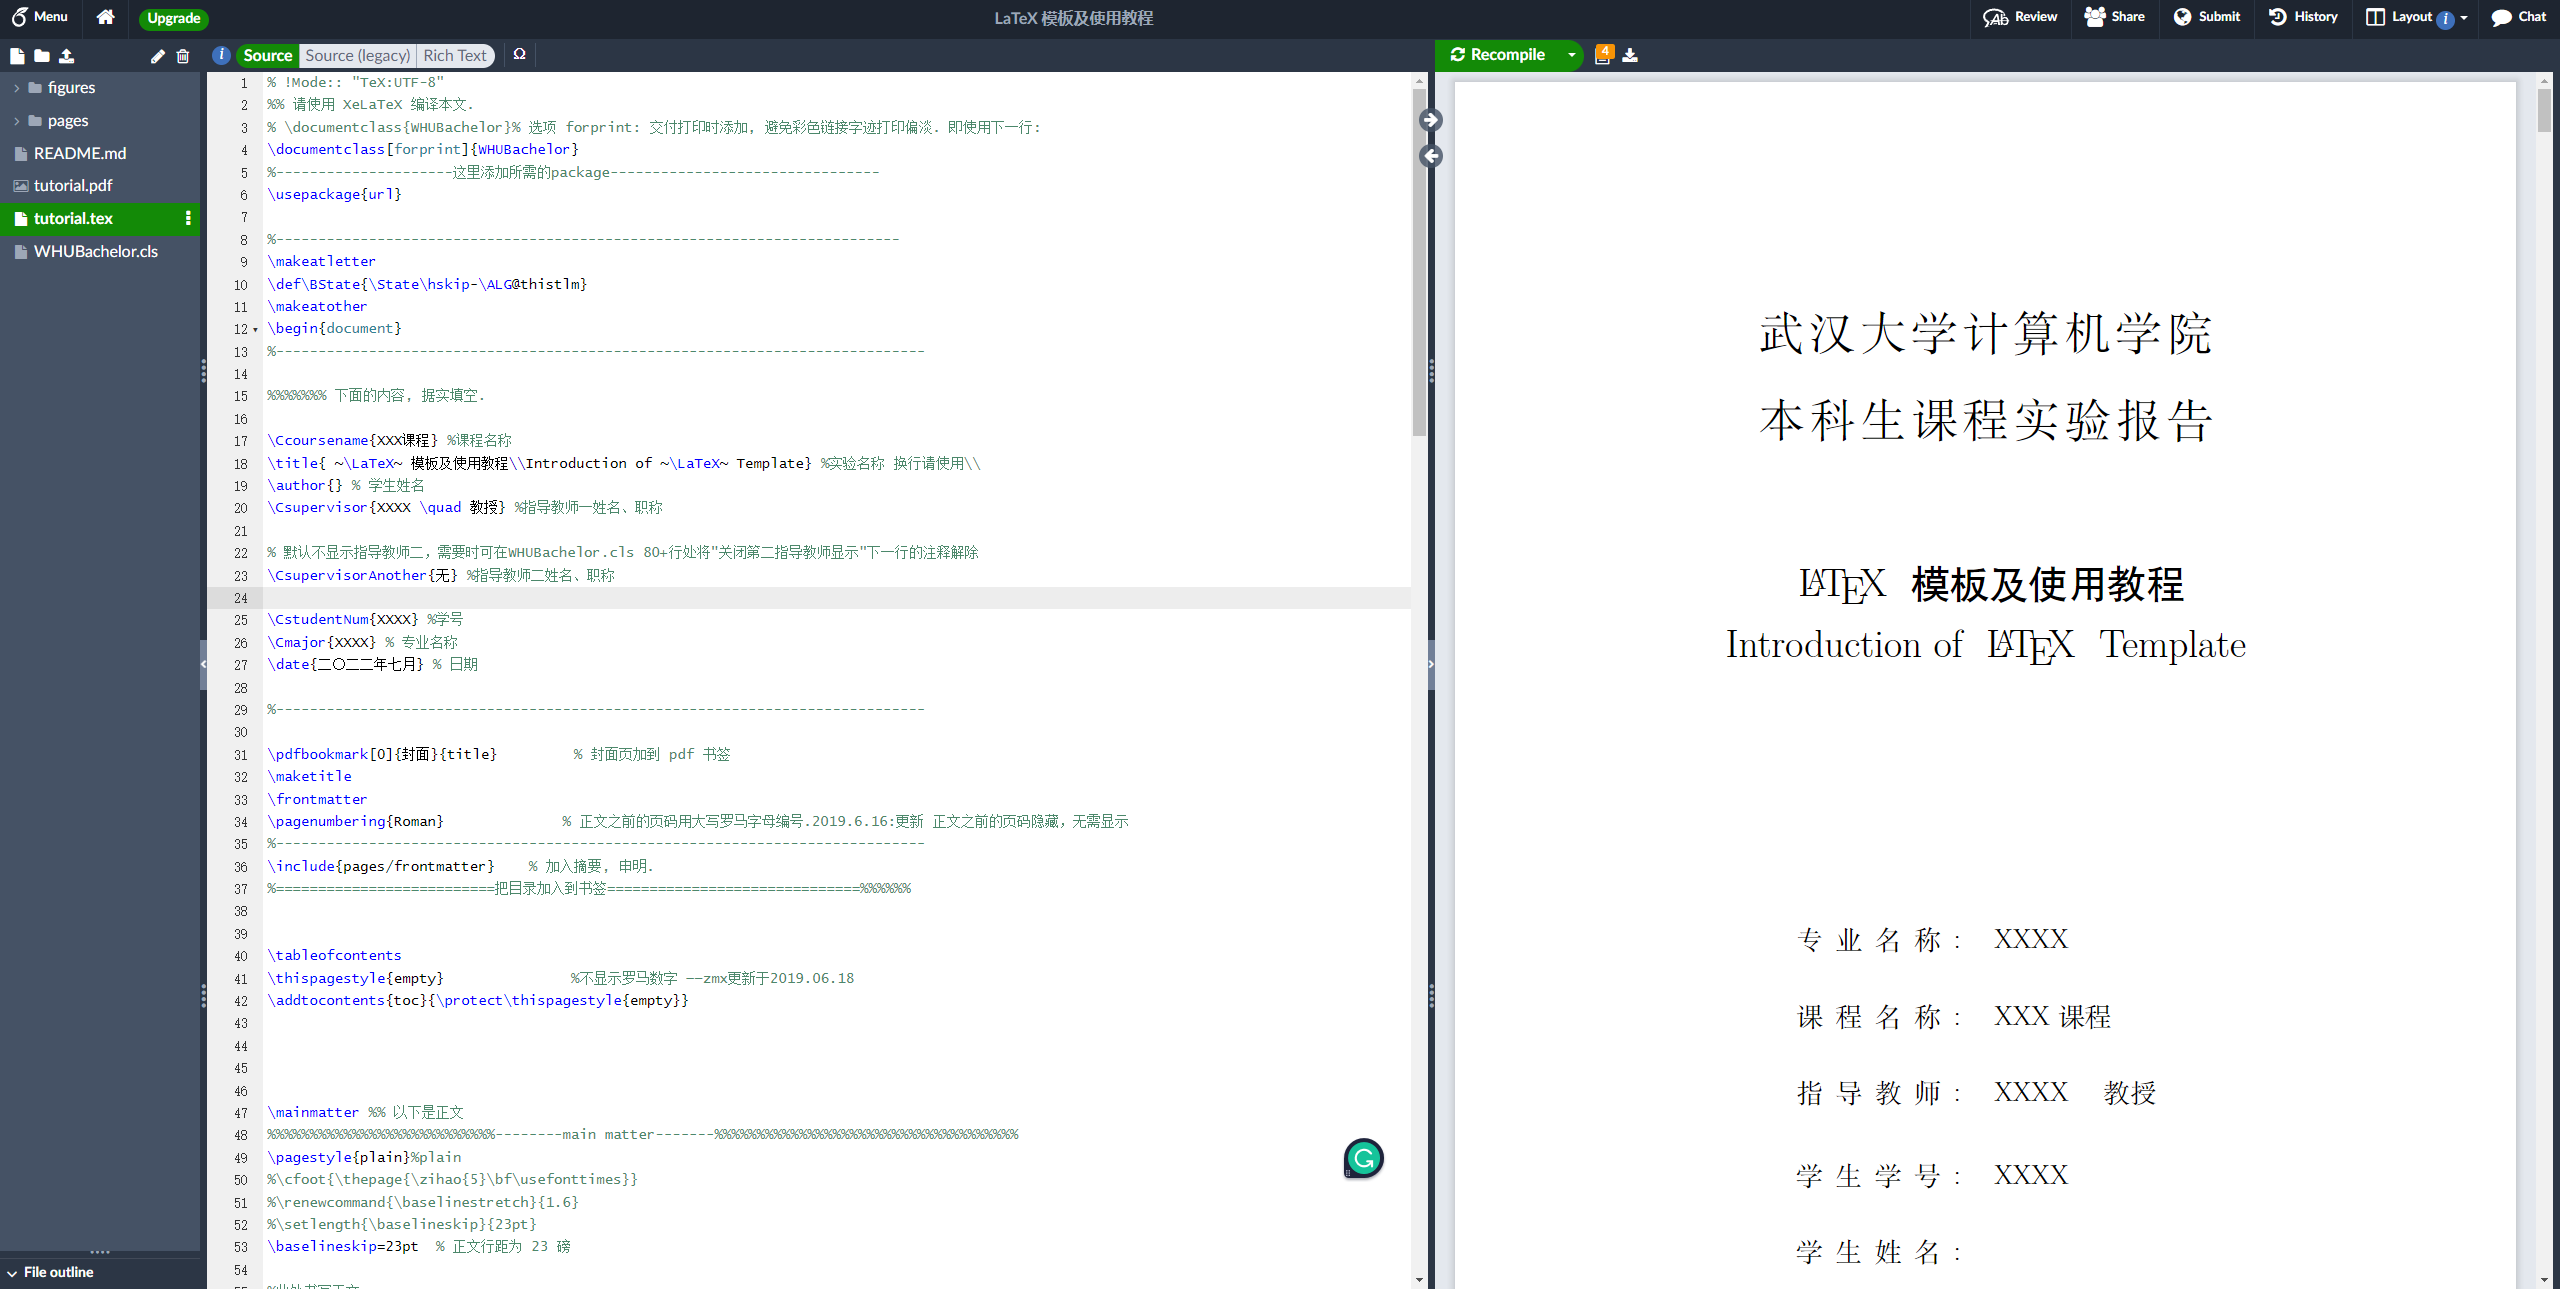
\includegraphics[width=0.95\textwidth]{figures/chapter2/overleaf-edit.png}
  \caption{Overleaf编辑页面}
  \label{fig:2-overleaf-edit}
\end{figure}

\section{本地编辑器}

\subsection{~\LaTeX~环境安装}

在清华源中下载Tex Live镜像文件:\url{https://mirrors.tuna.tsinghua.edu.cn/CTAN/systems/texlive/Images/texlive.iso},下载成功后双击挂载iso文件。


\begin{figure}[htb]
  \centering
  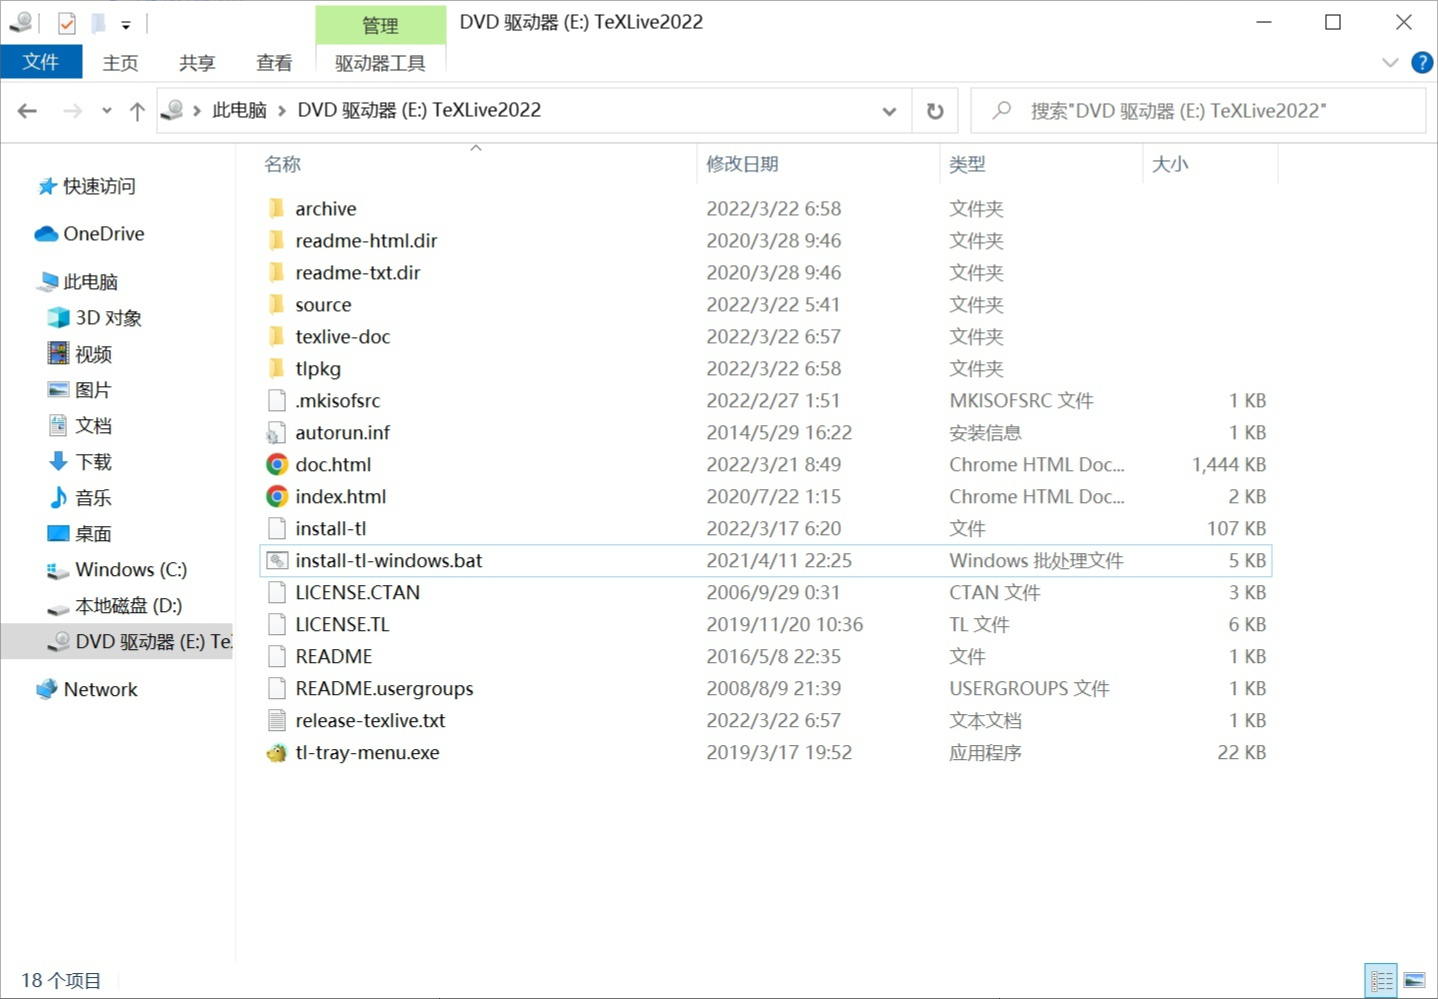
\includegraphics[width=0.95\textwidth]{figures/chapter2/texlive-iso.png}
  \caption{Tex Live镜像}
  \label{fig:2-texlive-iso}
\end{figure}

Windows下直接打开install-tl-windows.bat,Linux/Mac用户在终端下输入:

\begin{lstlisting}[language=bash]
  ./install-tl
\end{lstlisting}

使用默认配置进行安装。

\begin{figure}[htb]
  \centering
  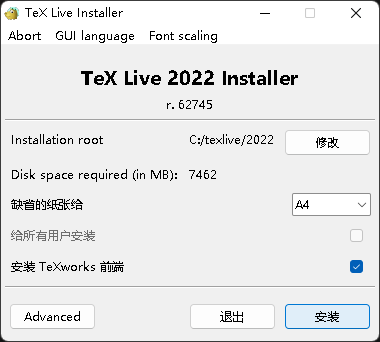
\includegraphics[width=0.4\textwidth]{figures/chapter2/texlive-install.png}
  \caption{Tex Live安装}
  \label{fig:2-texlive-install}
\end{figure}

详细安装过程和注意事项请参考:\url{https://github.com/OsbertWang/install-latex-guide-zh-cn/releases/latest/}

\subsection{VSCode配置}

Tex Live自带的编辑器不太好用,个人一般使用VSCode配合LaTeX Workshop插件。

\begin{enumerate}
  \item 点击拓展图标,打开拓展
  \item 输入"latex workshop",选择第一个LaTeX Workshop插件
  \item 点击"install"进行安装,等待安装完成(如图\ref{fig:2-plugin-install})
\end{enumerate}

\begin{figure}[H]
  \centering
  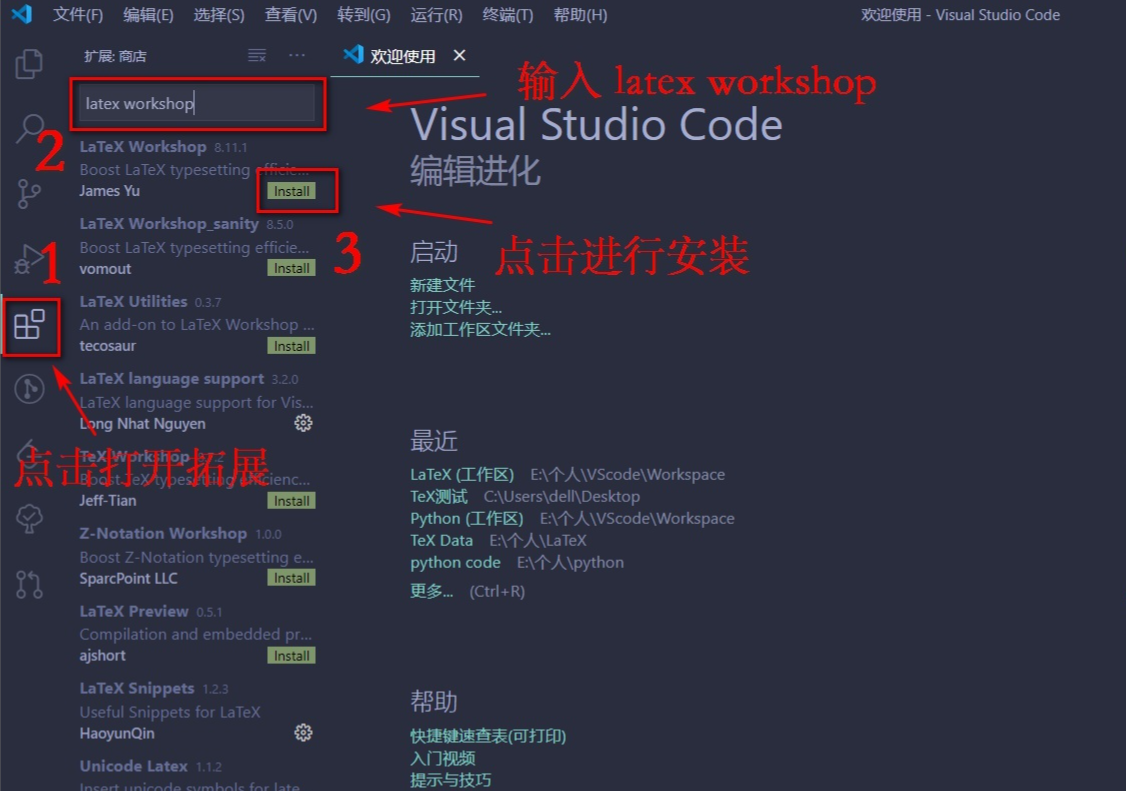
\includegraphics[width=0.95\textwidth]{figures/chapter2/plugin-install.png}
  \caption{LaTeX Workshop插件安装}
  \label{fig:2-plugin-install}
\end{figure}

\begin{enumerate}
  \item 点击设置图标
  \item 点击设置
  \item 转到 UI 设置页面(如图\ref{fig:2-vscode-settings})
  \item 点击右上侧图标打开JSON配置文件,进入代码设置页面(如图\ref{fig:2-vscode-json})
\end{enumerate}

\begin{figure}[H]
  \centering
  \begin{subfigure}{0.45\textwidth}
    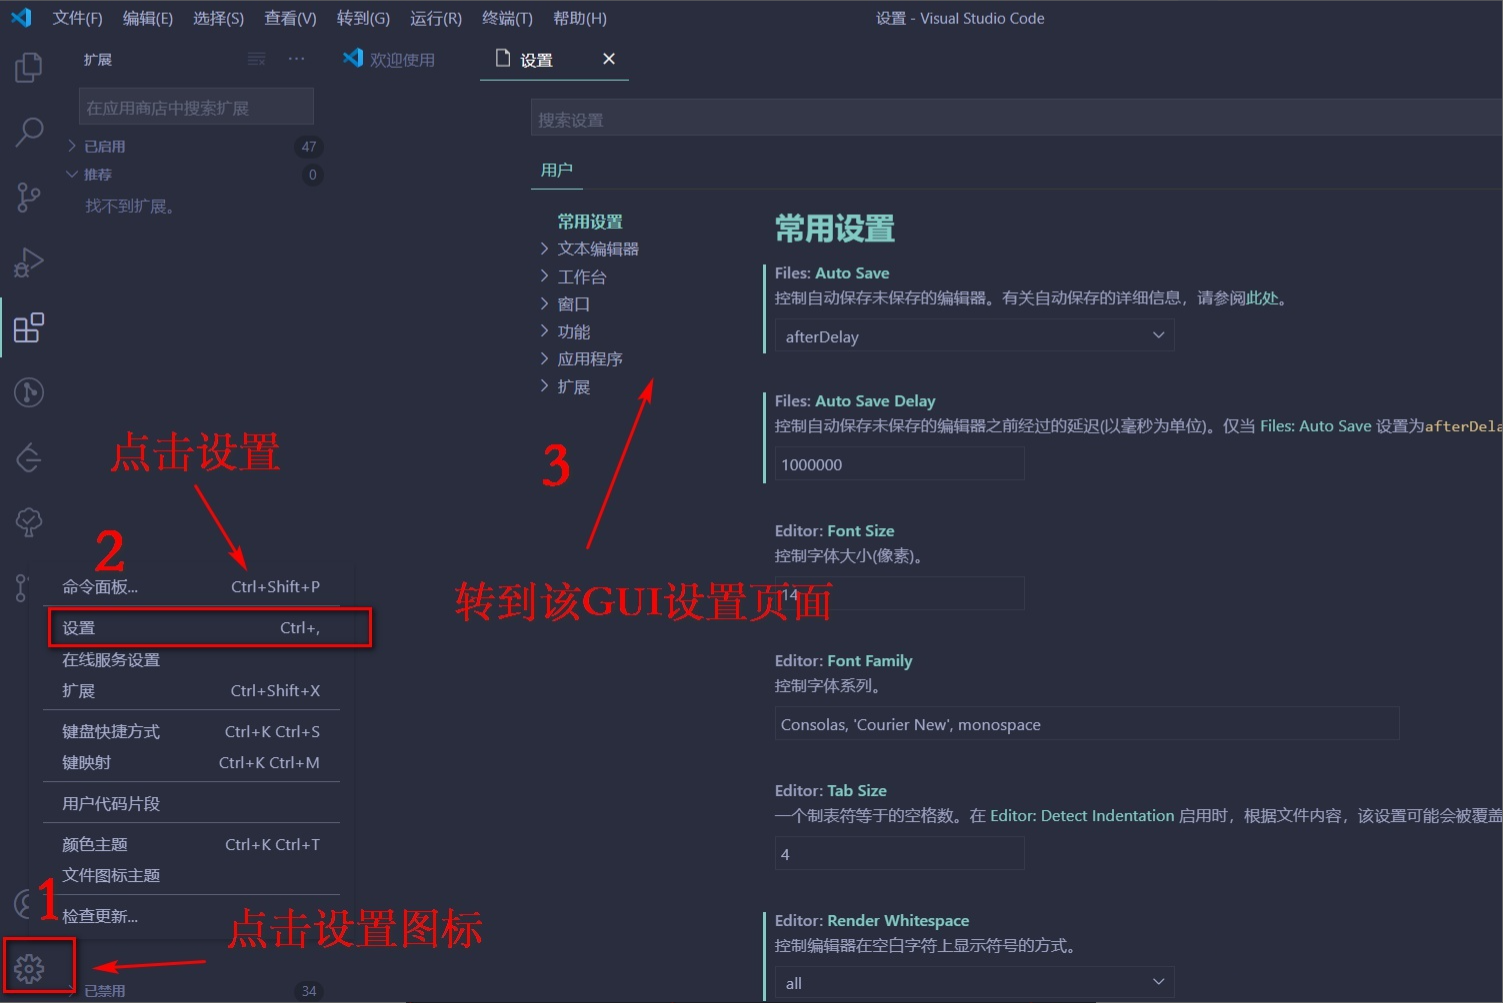
\includegraphics[width=\linewidth]{figures/chapter2/vscode-settings.png}
    \caption{UI设置界面}
    \label{fig:2-vscode-settings}
  \end{subfigure}\qquad
  \begin{subfigure}{0.45\textwidth}
    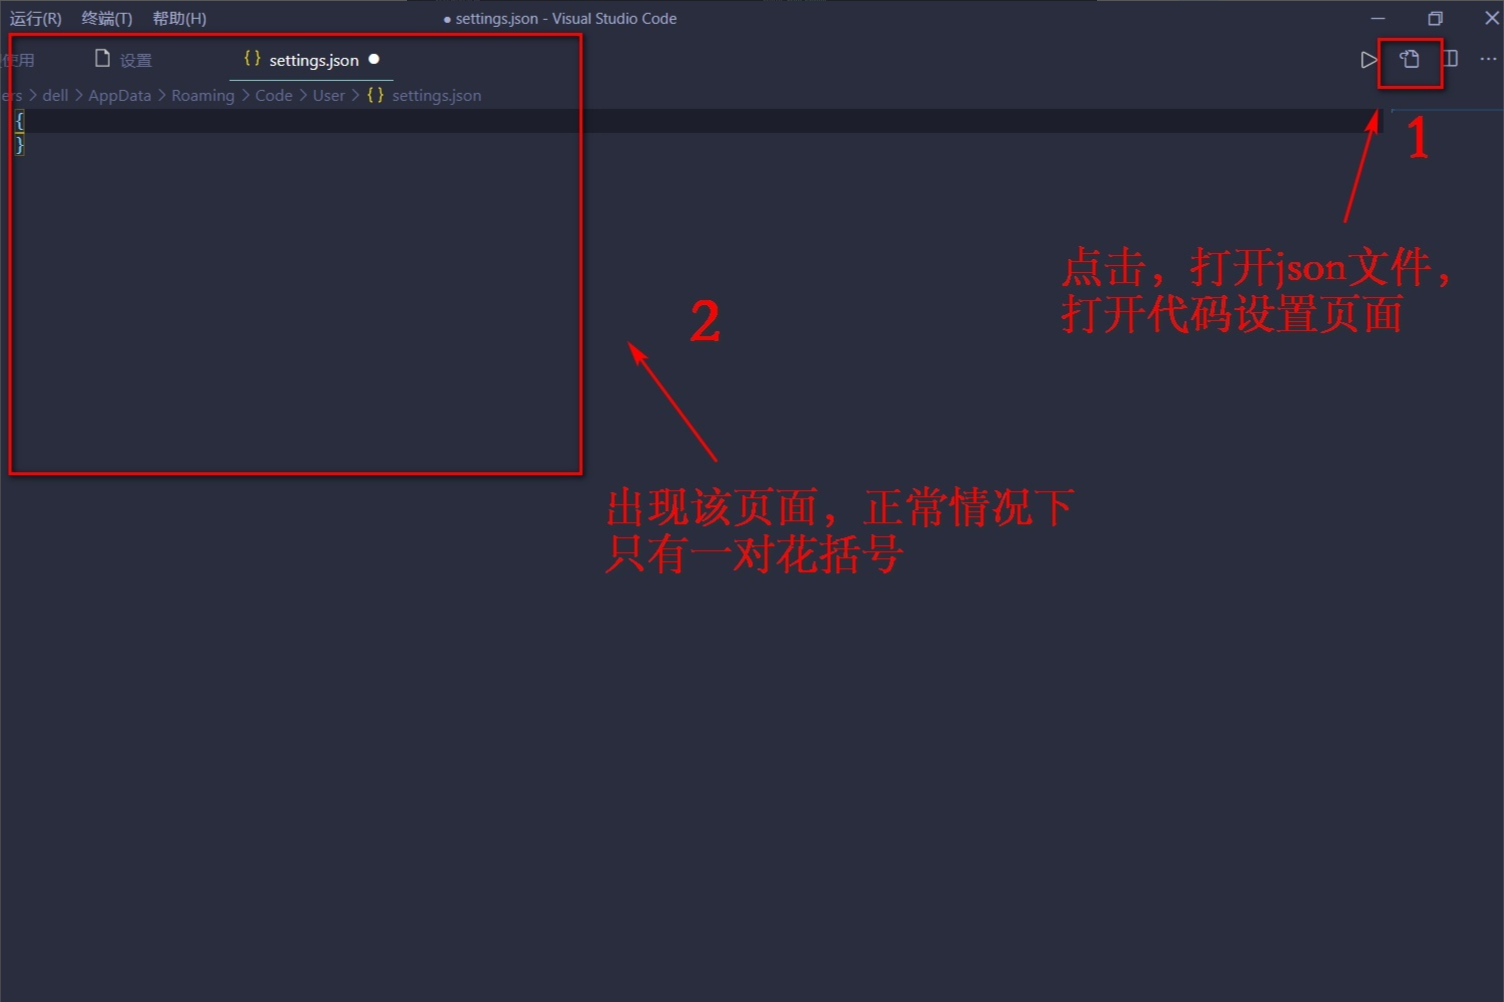
\includegraphics[width=\linewidth]{figures/chapter2/vscode-json.png}
    \caption{JSON配置文件}
    \label{fig:2-vscode-json}
  \end{subfigure}
  \caption{配置~\LaTeX~}
  \label{fig:2-vscode-conf}
\end{figure}

在JSON文件内输入以下内容:

由于PDF内代码不好复制,JSON内容请参考:\url{https://zhuanlan.zhihu.com/p/166523064}\quad \textbf{6.1 LaTeX配置代码展示}处

\begin{lstlisting}[language=json]
  {
    "latex-workshop.latex.autoBuild.run": "never",
    "latex-workshop.showContextMenu": true,
    "latex-workshop.intellisense.package.enabled": true,
    "latex-workshop.message.error.show": false,
    "latex-workshop.message.warning.show": false,
    "latex-workshop.latex.tools": [
        {
            "name": "xelatex",
            "command": "xelatex",
            "args": [
                "-synctex=1",
                "-interaction=nonstopmode",
                "-file-line-error",
                "%DOCFILE%"
            ]
        },
        {
            "name": "pdflatex",
            "command": "pdflatex",
            "args": [
                "-synctex=1",
                "-interaction=nonstopmode",
                "-file-line-error",
                "%DOCFILE%"
            ]
        },
        {
            "name": "latexmk",
            "command": "latexmk",
            "args": [
                "-synctex=1",
                "-interaction=nonstopmode",
                "-file-line-error",
                "-pdf",
                "-outdir=%OUTDIR%",
                "%DOCFILE%"
            ]
        },
        {
            "name": "bibtex",
            "command": "bibtex",
            "args": [
                "%DOCFILE%"
            ]
        }
    ],
    "latex-workshop.latex.recipes": [
        {
            "name": "XeLaTeX",
            "tools": [
                "xelatex"
            ]
        },
        {
            "name": "PDFLaTeX",
            "tools": [
                "pdflatex"
            ]
        },
        {
            "name": "BibTeX",
            "tools": [
                "bibtex"
            ]
        },
        {
            "name": "LaTeXmk",
            "tools": [
                "latexmk"
            ]
        },
        {
            "name": "xelatex -> bibtex -> xelatex*2",
            "tools": [
                "xelatex",
                "bibtex",
                "xelatex",
                "xelatex"
            ]
        },
        {
            "name": "pdflatex -> bibtex -> pdflatex*2",
            "tools": [
                "pdflatex",
                "bibtex",
                "pdflatex",
                "pdflatex"
            ]
        },
    ],
    "latex-workshop.latex.clean.fileTypes": [
        "*.aux",
        "*.bbl",
        "*.blg",
        "*.idx",
        "*.ind",
        "*.lof",
        "*.lot",
        "*.out",
        "*.toc",
        "*.acn",
        "*.acr",
        "*.alg",
        "*.glg",
        "*.glo",
        "*.gls",
        "*.ist",
        "*.fls",
        "*.log",
        "*.fdb_latexmk"
    ],
    "latex-workshop.latex.autoClean.run": "onFailed",
    "latex-workshop.latex.recipe.default": "lastUsed",
    "latex-workshop.view.pdf.internal.synctex.keybinding": "double-click"
}
\end{lstlisting}

\subsection{VSCode编译}

此时你需要将使用的模板下载至本地。以此项目为例,进入\url{https://github.com/Nagico/WHUExperiment},点击Download ZIP即可将模板下载到本地。该模板同时也一同放至本文档旁,可以直接使用,但仍建议从Github上下载最新版本的模板。

\begin{figure}[htb]
  \centering
  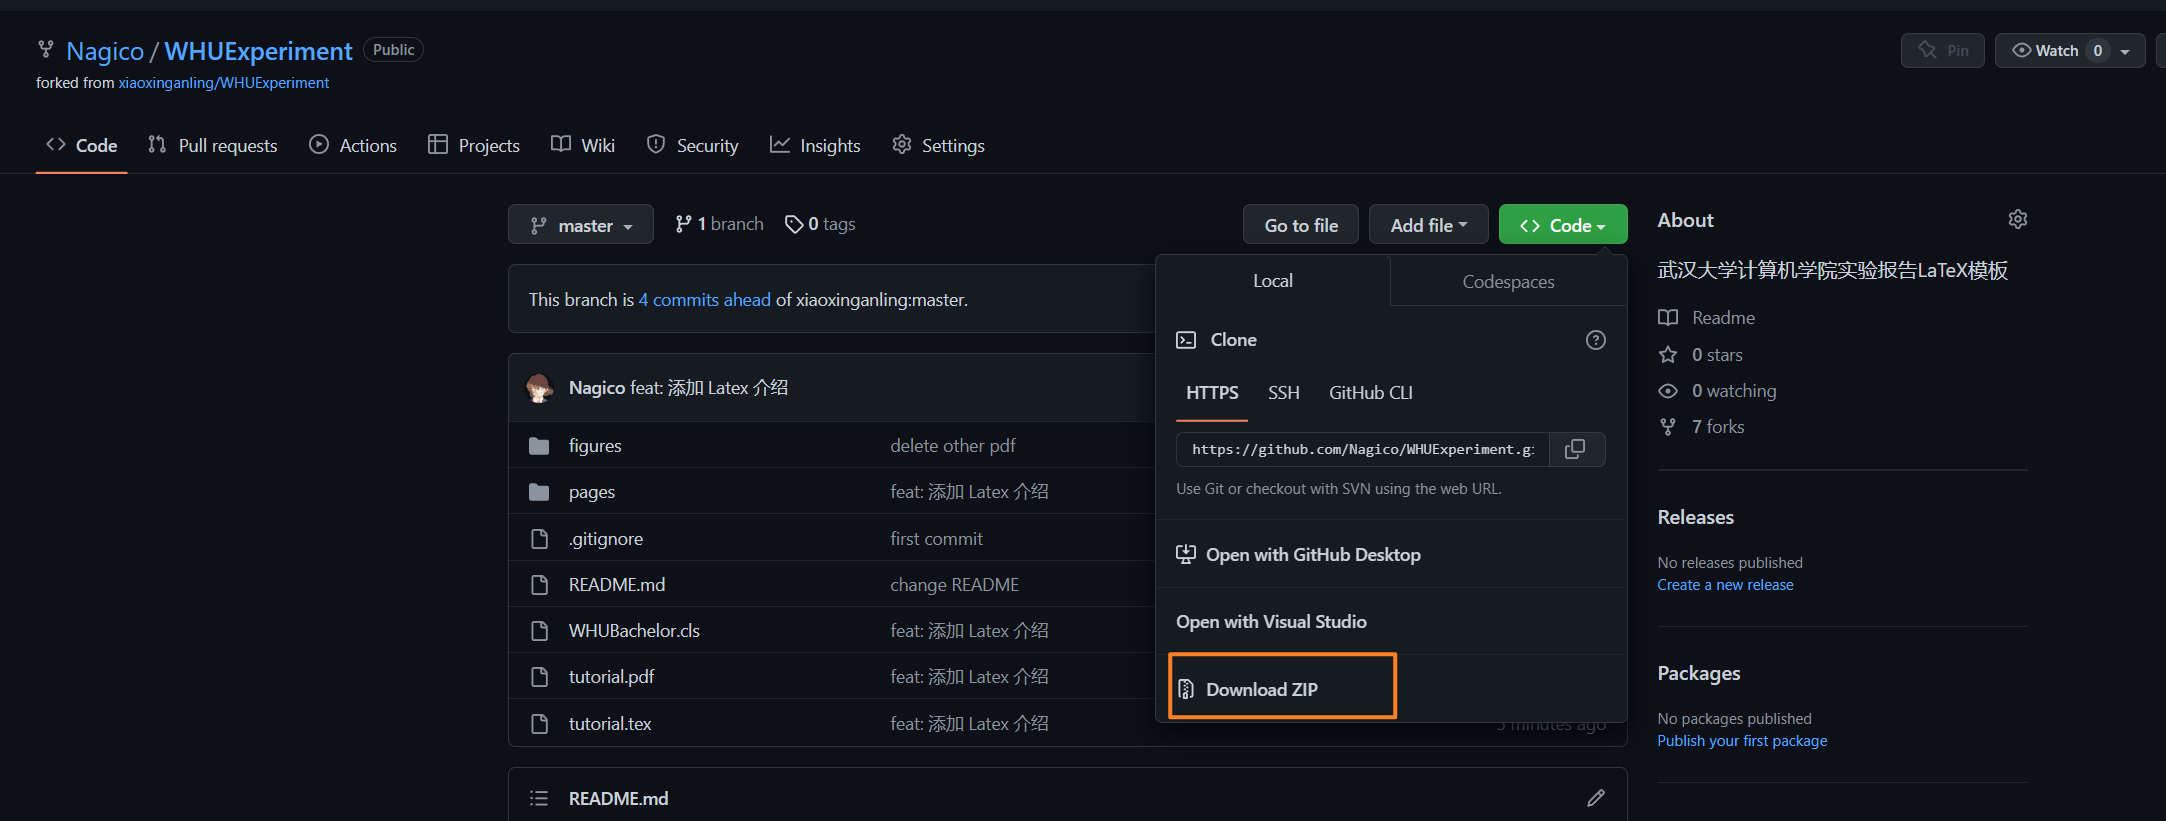
\includegraphics[width=0.95\textwidth]{figures/chapter2/download-repo.png}
  \caption{下载模板}
  \label{fig:2-github-download-2}
\end{figure}

将项目解压后用VSCode打开文件夹,点击选中 tex 文件,进行文件内容查看。

\begin{figure}[H]
  \centering
  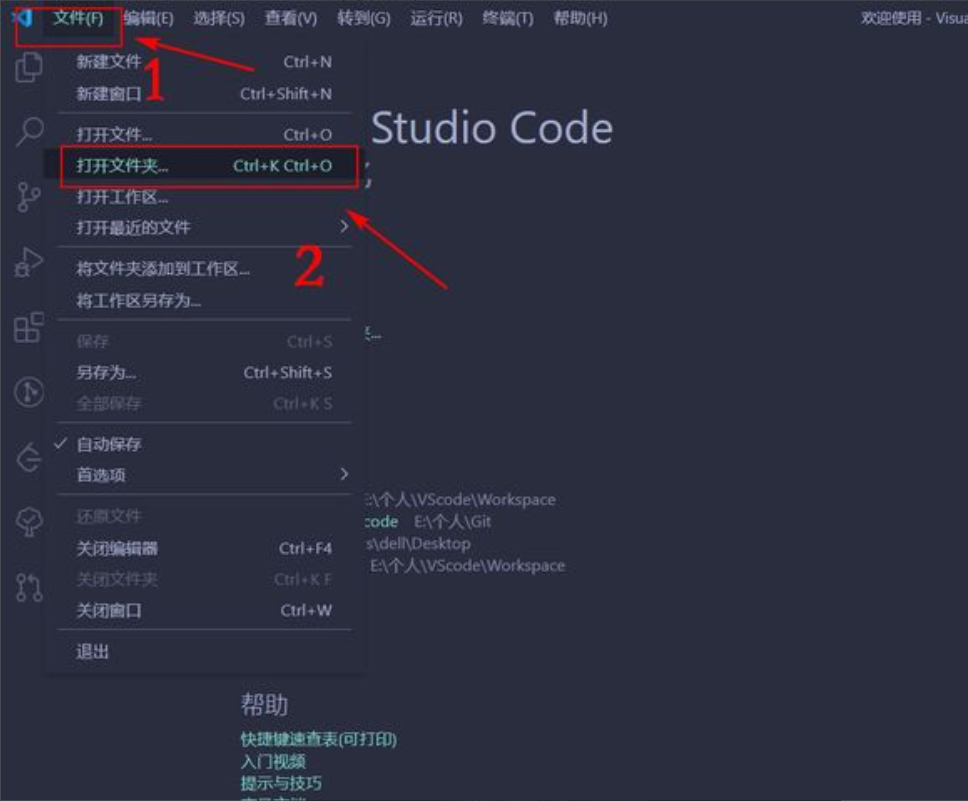
\includegraphics[width=0.9\textwidth]{figures/chapter2/vscode-open.png}
  \caption{打开项目文件夹}
  \label{fig:2-vscode-open-folder}
\end{figure}

\begin{figure}[H]
  \centering
  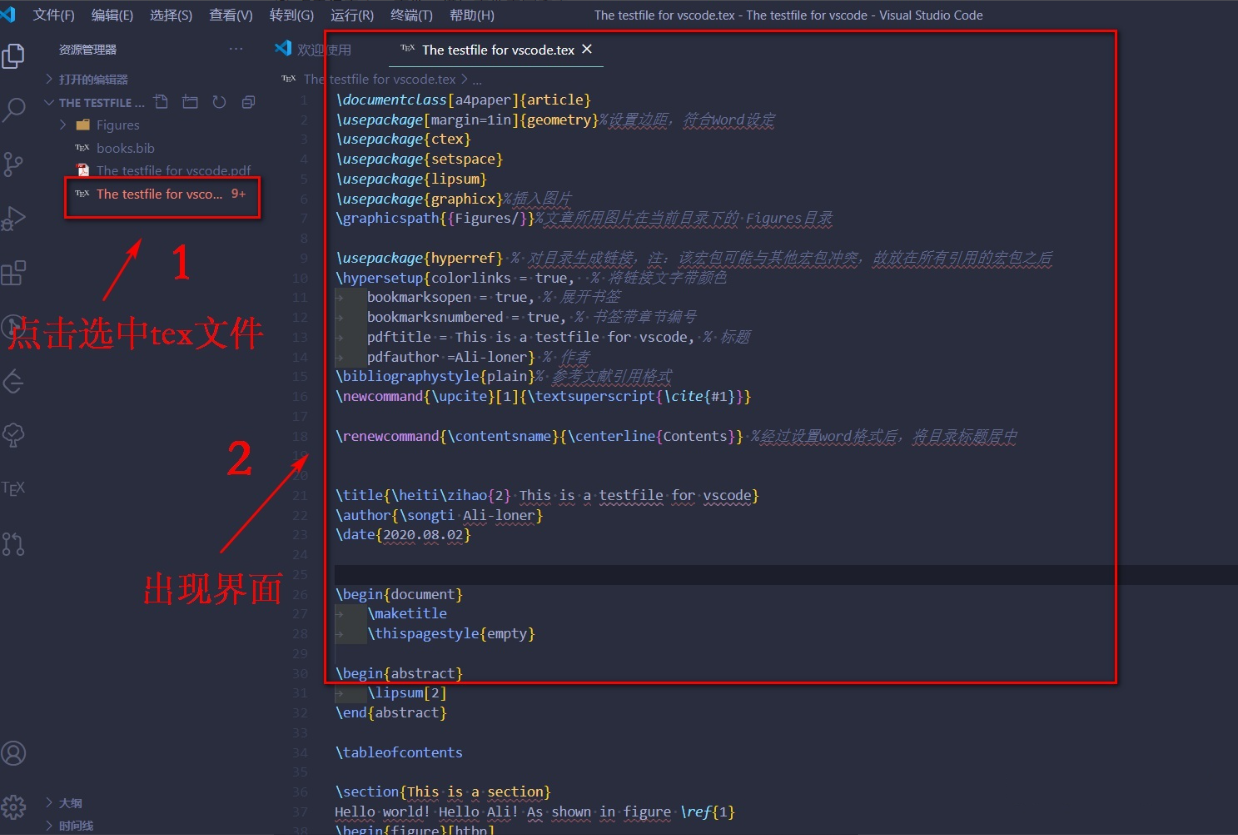
\includegraphics[width=0.9\textwidth]{figures/chapter2/vscode-openfile.png}
  \caption{打开Tex文件}
  \label{fig:2-vscode-open-file}
\end{figure}

由于项目中会涉及参考文献的引用(.bib的编译),故而选择xelatex -> bibtex -> xelatex*2编译链。

\begin{figure}[htb]
  \centering
  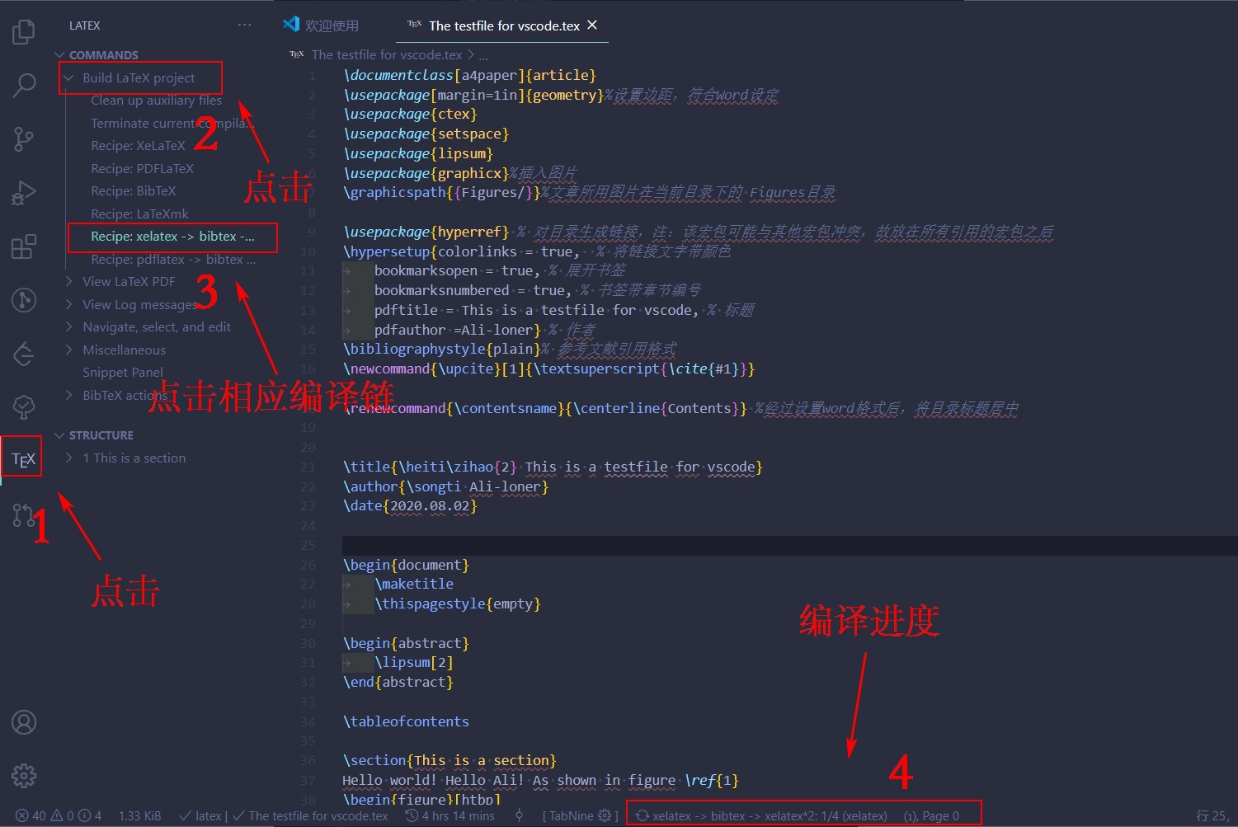
\includegraphics[width=0.8\textwidth]{figures/chapter2/vscode-compile.png}
  \caption{Tex编译}
  \label{fig:2-vscode-tex-compile}
\end{figure}

点击编辑界面的右上角图标,即可查看编译结果。

\begin{figure}[H]
  \centering
  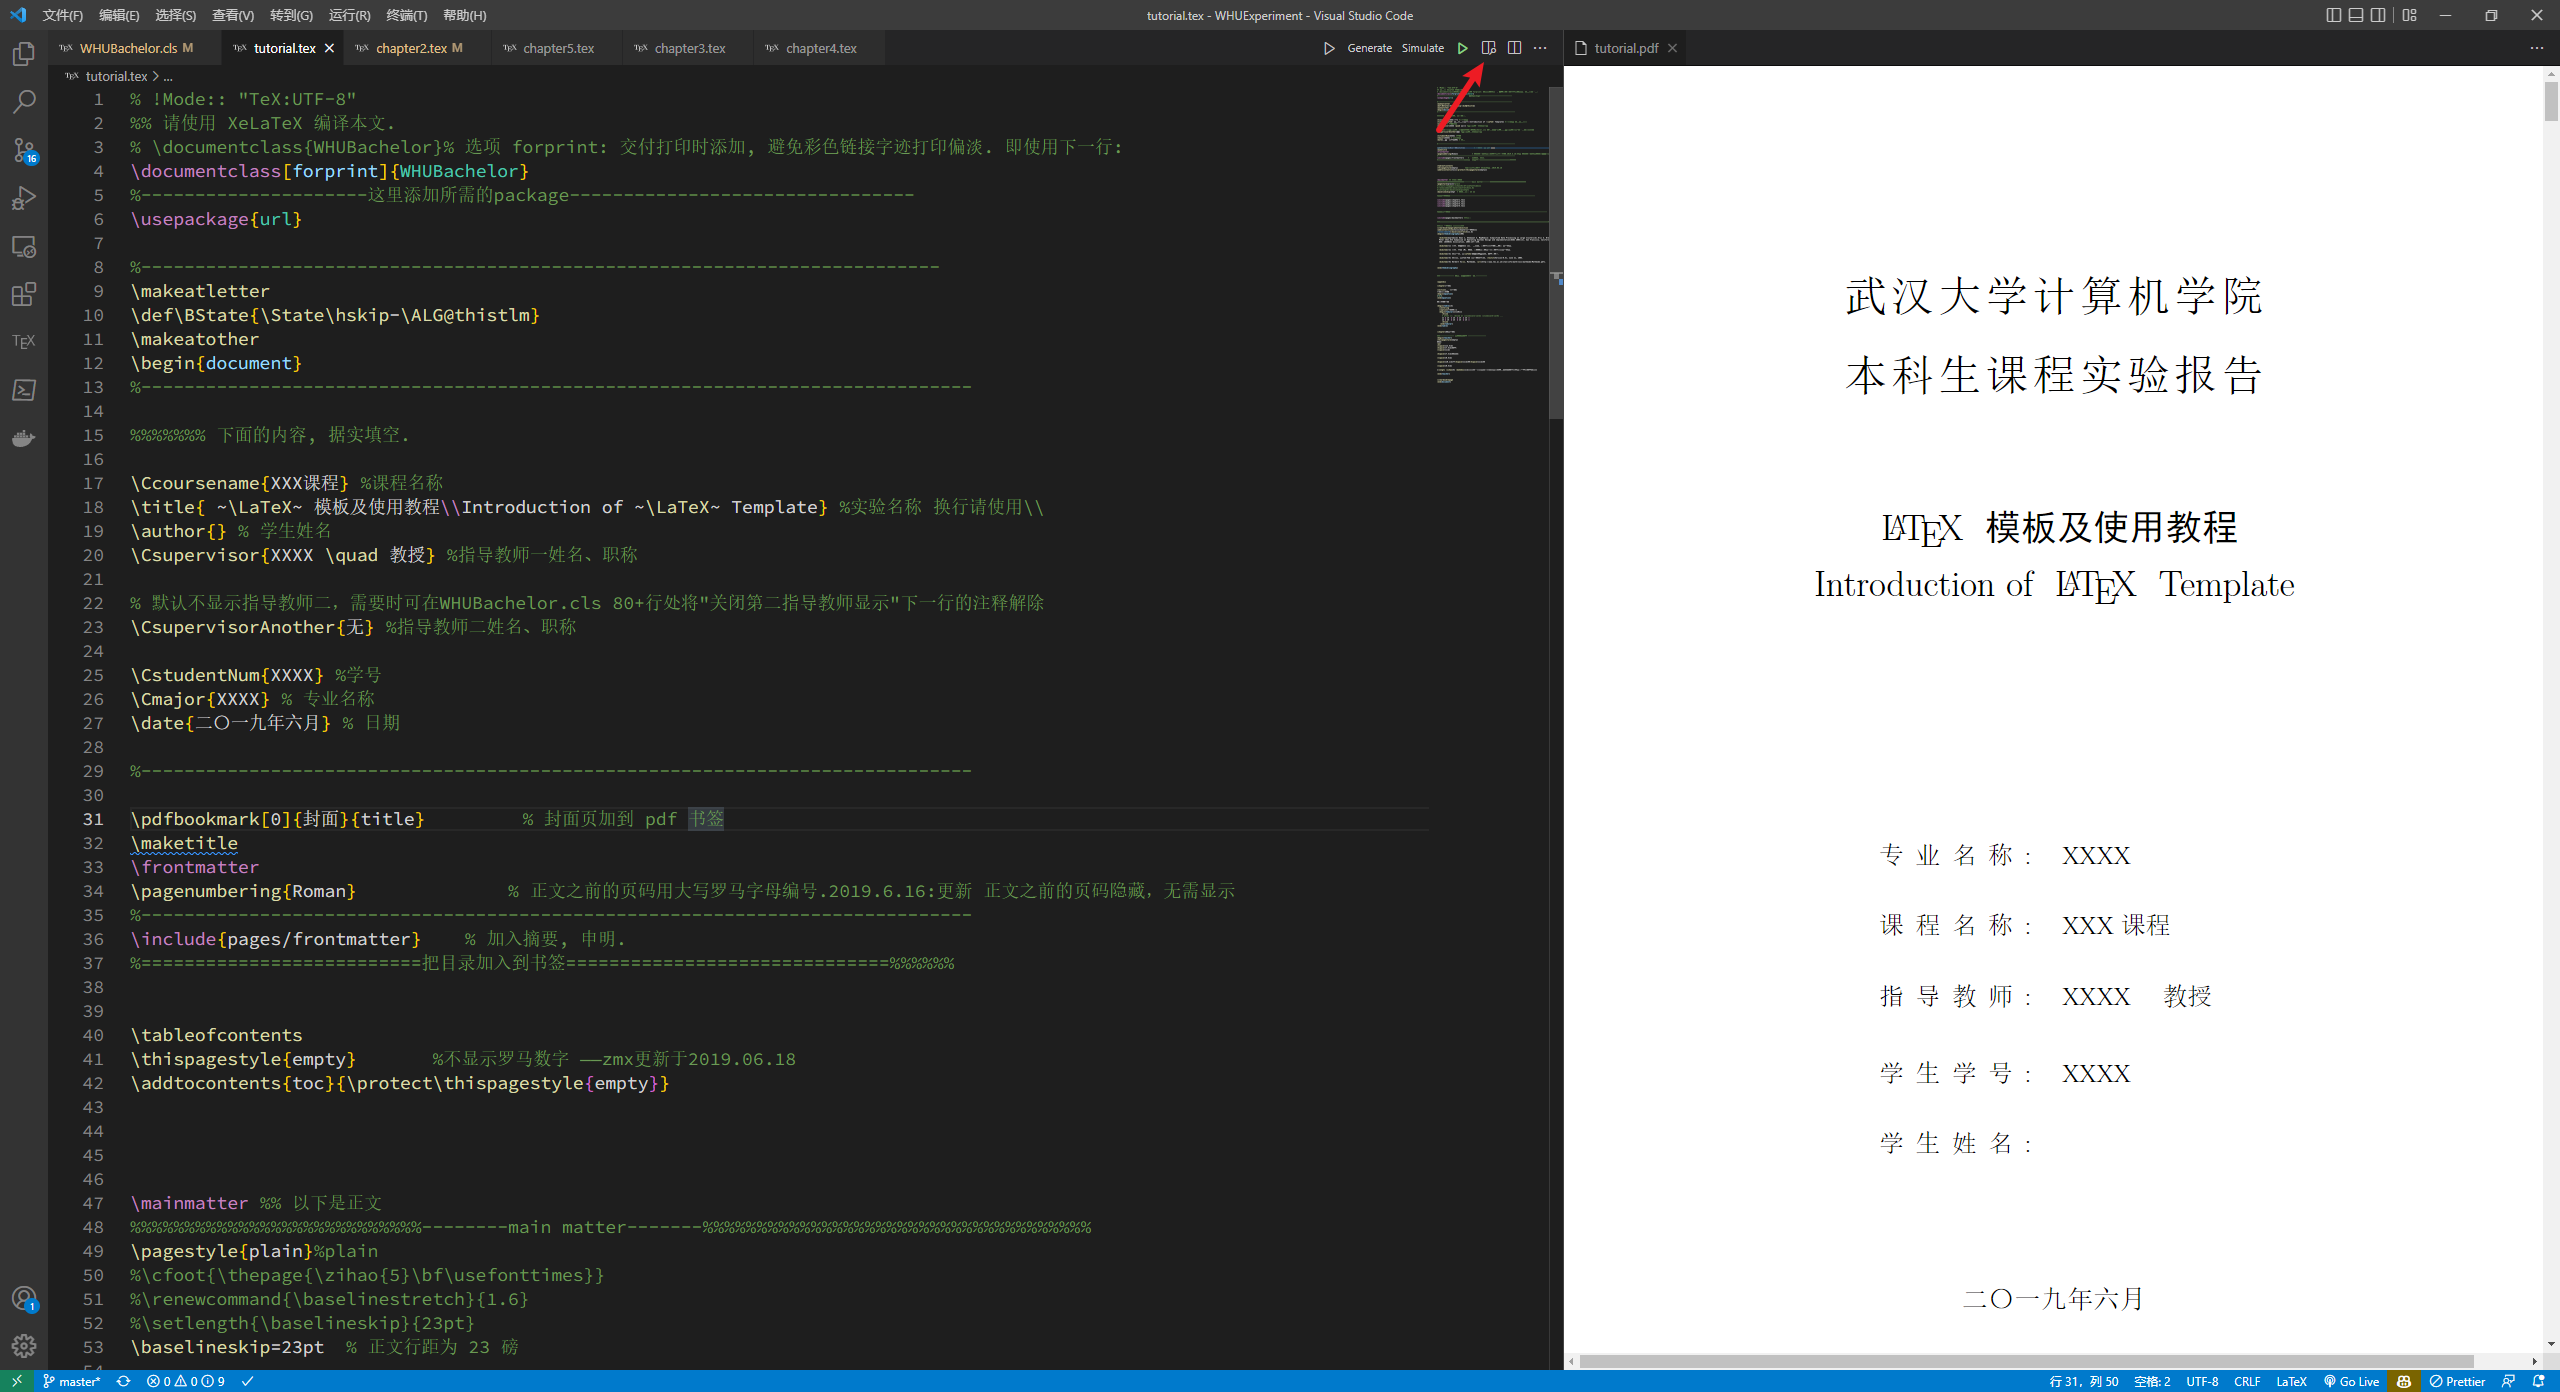
\includegraphics[width=0.95\textwidth]{figures/chapter2/vscode-edit.png}
  \caption{Tex编译结果}
  \label{fig:2-vscode-edit}
\end{figure}

更多VSCode配置可参考网上Blog,实现双向自动跳转等功能。新版VSCode、插件与以前有一定差别,最好选择2022年及以后较新的Blog学习。